% Page-anchored objects with real column-height reservations (no overlays).
% Current draft: Fig.2 p2 upper-right; Table I p2 lower-right;
% Fig.3 p3 top-wide; Table II p4 top-wide. Body copy stays in reading order.
\newif\ifpaperfixedpages
\iflayoutdraft\paperfixedpagestrue\else\paperfixedpagesfalse\fi
\newsavebox{\paperfigtwobox}
\newsavebox{\papertableonebox}
\newsavebox{\paperfigthreebox}
\newsavebox{\papertabletwobox}
\newlength{\paperfixedgap}
\setlength{\paperfixedgap}{8pt}
\makeatletter
\newcommand{\paperpreparefixedobjects}{%
  \ifpaperfixedpages
    \begingroup
      \setcounter{figure}{1}%
      \global\setbox\paperfigtwobox=\vbox{\hsize\columnwidth\linewidth\columnwidth
        \normalfont\normalsize\begin{paperfigure}
% One native vector drawing; both panels use identical geometry and typography.
% Final size: 252 x 157 pt, matching one IEEE column without shrinking text.
\begingroup
\definecolor{rfInk}{HTML}{182838}
\definecolor{rfMuted}{HTML}{657382}
\definecolor{rfGuide}{HTML}{AAB5BF}
\definecolor{rfMemory}{HTML}{6E52A2}
\definecolor{rfCompute}{HTML}{178E9D}
\newcommand{\rfFont}{\fontencoding{OT1}\fontfamily{DejaVuSans-TLF}\selectfont}
% Greek letters use the same DejaVu Sans family as the Latin labels and Python
% plots. This local text-font selection does not change manuscript math fonts.
\newcommand{\rfGreek}[1]{{\fontencoding{LGR}\fontshape{it}\selectfont#1}}
\newcommand{\rfPi}{\rfGreek{\textpi}}
\newcommand{\rfBeta}{\rfGreek{\textbeta}}
\newcommand{\rfRho}{\rfGreek{\textrho}}
\newcommand{\rfTau}{\rfGreek{\texttau}}
% Arguments: x shift, heading, y label, x label, ceiling, slope, ridge,
% left regime, right regime. Each panel deliberately uses its own linear scales.
\newcommand{\rooflinepanel}[9]{%
  \begin{scope}[xshift=#1]
    \node[font=\rfFont\fontsize{7.4}{8.4}\selectfont\bfseries]
      at (72,149) {#2};
    \fill[rfMemory!7] (25,59) -- (65,118) -- (65,59) -- cycle;
    \fill[rfCompute!7] (65,59) rectangle (119,118);
    \draw[rfguide] (25,118) -- (65,118);
    \draw[rfguide] (65,59) -- (65,118);
    \draw[rfaxis] (25,59) -- (122,59);
    \draw[rfaxis] (25,59) -- (25,136);
    \draw[rfMemory,line width=1.6pt,line cap=round]
      (25,59) -- (65,118)
      node[midway,above=3pt,sloped,text=rfMemory,
           font=\rfFont\fontsize{6.5}{7.5}\selectfont] {slope #6};
    \draw[rfCompute,line width=1.6pt,line cap=round]
      (65,118) -- (119,118);
    \fill[rfInk] (65,118) circle[radius=1.7pt];
    \node[text=rfCompute,font=\rfFont\fontsize{6.5}{7.5}\selectfont]
      at (92,126) {ceiling #5};
    \node[anchor=east] at (21,118) {#5};
    \node[rotate=90] at (8,98) {#3};
    \draw[rfMuted,line width=.6pt] (65,59) -- (65,56.5);
    \node[font=\rfFont\fontsize{6.7}{7.7}\selectfont] at (65,49) {#7};
    \node[align=center,text=rfMemory,
          font=\rfFont\fontsize{6.5}{7.5}\selectfont]
      at (44,33) {#8-\\bound};
    \node[align=center,text=rfCompute,
          font=\rfFont\fontsize{6.5}{7.5}\selectfont]
      at (94,33) {#9-\\bound};
    \node[align=center,font=\rfFont\fontsize{6.7}{7.8}\selectfont]
      at (72,11) {#4};
  \end{scope}%
}
\begin{tikzpicture}[
  x=1pt,y=1pt,
  every node/.style={font=\rfFont\fontsize{7.2}{8.2}\selectfont,
                    text=rfInk,inner sep=.5pt,outer sep=0pt},
  rfaxis/.style={draw=rfMuted,line width=.65pt,
                -{Stealth[length=3pt,width=3pt]}},
  rfguide/.style={draw=rfGuide,line width=.55pt,dash pattern=on 2pt off 2pt}
]
  \path[use as bounding box] (0,0) rectangle (252,157);
  \rooflinepanel{0pt}{(a) Classical}
    {\textit{P}\textsubscript{OP} [OP/s]}
    {Arithmetic intensity\\AI [OP/Byte]}
    {\rfPi}{\rfBeta}
    {AI\textsuperscript{*} = \rfPi/\rfBeta}
    {Memory}{Compute}
  \rooflinepanel{128pt}{(b) Resident-streaming}
    {\textit{P} [Byte/s]}
    {Resident intensity\\RI [Byte/Byte]}
    {\rfRho}{\rfTau}
    {RI\textsuperscript{*} = \rfRho/\rfTau}
    {Resident}{Streaming}
\end{tikzpicture}
\endgroup

\caption{Classical GPU~\cite{williams2009roofline} and resident-streaming CIM Rooflines with their accounting correspondence. Panels use independent linear scales; curves are upper bounds. OP and Byte denote operation and transferred-byte counts.}
\label{fig:roofline-comparison}
\end{paperfigure}
\unskip}%
      \setcounter{table}{0}%
      \global\setbox\papertableonebox=\vbox{\hsize\columnwidth\linewidth\columnwidth
        \normalfont\normalsize% Selected from Task II(a) data/results.json; exact values in selected_reuse.csv.
\begin{papertable}
\caption{Resident intensity after one complete weight load}
\label{tab:reuse-intensity}
\footnotesize\setlength{\tabcolsep}{2.5pt}\renewcommand{\arraystretch}{1.15}
\begin{tabularx}{\columnwidth}{@{}l*{6}{>{\centering\arraybackslash}X}@{}}
\toprule
Weight shape & \multicolumn{6}{c}{Reuse count $U$} \\
\cmidrule(l){2-7}
$N\times K$ & $128$ & $1\Kilo$ & $16\Kilo$ & $128\Kilo$ & $1\mathrm{M}$ & $\to\infty$ \\
\midrule
$128\times128$ & 1.0 & 8.0 & 128.0 & 1024.0 & 8192.0 & $\infty$ \\
$1024\times1024$ & 0.125 & 1.0 & 16.0 & 128.0 & 1024.0 & $\infty$ \\
$4096\times4096$ & 0.0313 & 0.250 & 4.0 & 32.0 & 256.0 & $\infty$ \\
$1024\times4096$ & 0.125 & 1.0 & 16.0 & 128.0 & 1024.0 & $\infty$ \\
$4096\times1024$ & 0.0313 & 0.250 & 4.0 & 32.0 & 256.0 & $\infty$ \\
\bottomrule\end{tabularx}
\par\smallskip\raggedright
One byte/element: $Q_S=UK$, $Q_R=NK$, $\RI=U/N$. As $U\to\infty$, the single load $Q_R=NK$ stays finite. Shapes are logical matrices, not hardware tiles. $1\Kilo=1024$, $1\mathrm{M}=1024^2$.
\end{papertable}
\unskip}%
      \setcounter{figure}{2}%
      \global\setbox\paperfigthreebox=\vbox{\hsize\textwidth\linewidth\textwidth
        \normalfont\normalsize\begin{paperwidefigure}
% Submission typography; original vector and all geometry retained separately.
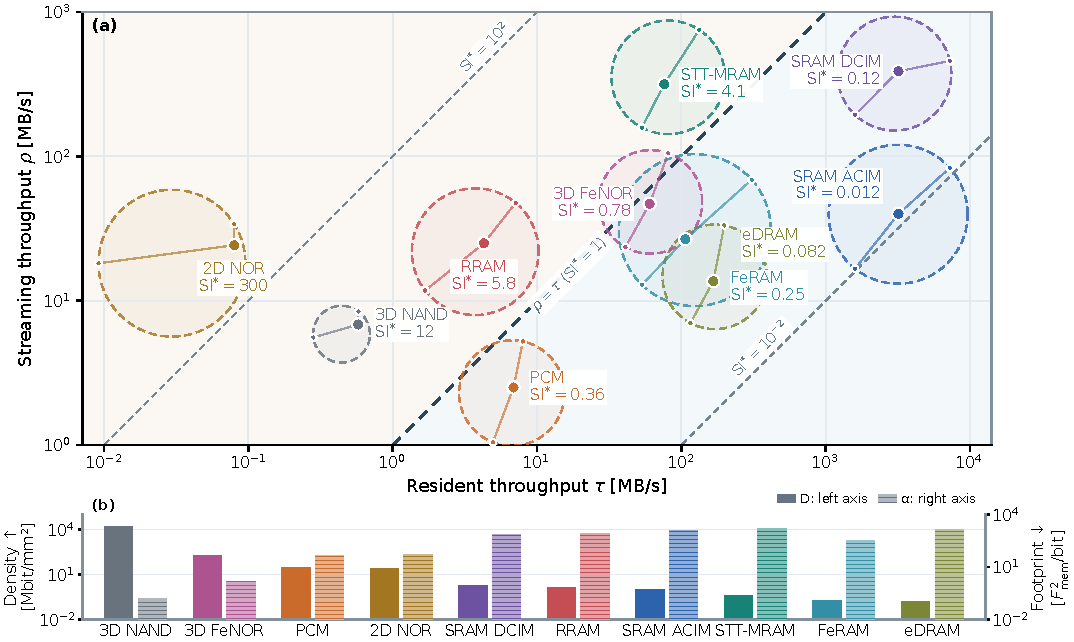
\includegraphics[width=\textwidth]{figures/hardware_capacities_paper.pdf}
\caption{Streaming capacity $\rho$ and resident-update capacity $\tau$ for ten native reference configurations; $1\ \mathrm{MB/s}=10^6\ \Byte/\mathrm{s}$. Large points are typical scenarios; small points preserve the original paired alternatives. Circles summarize only those finite scenarios, and $\RI^*=1$ is a capacity-ratio reference, not a universal workload boundary. Native sizes and resources differ.}
\label{fig:hardware-capacities}
\end{paperwidefigure}
\unskip}%
      \setcounter{table}{1}%
      \global\setbox\papertabletwobox=\vbox{\hsize\textwidth\linewidth\textwidth
        \normalfont\normalsize% Selected from Task II(b) 04_crosscheck/data/results.json; no O-projection values are implied.
\begin{paperwidetable}
\caption{Streaming intensities of representative inference matrix stages}
\label{tab:workload-intensity}
\footnotesize\setlength{\tabcolsep}{1.6pt}\renewcommand{\arraystretch}{1.25}
\begin{tabularx}{\textwidth}{@{}p{0.20\textwidth}*{12}{>{\centering\arraybackslash}X}@{}}
\toprule
& \multicolumn{6}{c}{\textbf{Weight projections}} & \multicolumn{6}{c}{\textbf{Attention}} \\
\cmidrule(lr){2-7}\cmidrule(l){8-13}
& \multicolumn{3}{c}{QKV ($U$)} & \multicolumn{3}{c}{FFN/MoE ($U$)} & \multicolumn{3}{c}{Prefill ($L$)} & \multicolumn{3}{c}{Decode ($L$)} \\
\cmidrule(lr){2-4}\cmidrule(lr){5-7}\cmidrule(lr){8-10}\cmidrule(l){11-13}
Model & $1\Kilo$ & $128\Kilo$ & $1\mathrm{M}$ & $16$ & $1\Kilo$ & $16\Kilo$ & $1\Kilo$ & $8\Kilo$ & $64\Kilo$ & $1\Kilo$ & $8\Kilo$ & $64\Kilo$ \\
\midrule
Qwen3.5-2B & 0.200 & 25.6 & 204.8 & 0.00347 & 0.222 & 3.6 & 6.0 & 34.0 & 258.0 & 10.0 & 66.0 & 514.0 \\
Ministral 3 8B & 0.167 & 21.3 & 170.7 & 0.00167 & 0.107 & 1.7 & 10.0 & 66.0 & 514.0 & 18.0 & 130.0 & 1026.0 \\
Qwen3.6-35B-A3B & 0.111 & 14.2 & 113.8 & 0.0130 & 0.833 & 13.3 & 12.0 & 68.0 & 516.0 & 20.0 & 132.0 & 1028.0 \\
Hy3 (295B) & 0.100 & 12.8 & 102.4 & 0.00477 & 0.306 & 4.9 & 20.0 & 132.0 & 1028.0 & 36.0 & 260.0 & 2052.0 \\
Ling-1T (1000B) & 0.100 & 12.8 & 102.4 & 0.00326 & 0.208 & 3.3 & 20.0 & 132.0 & 1028.0 & 36.0 & 260.0 & 2052.0 \\
MiMo-V2.5-Pro (1020B) & 0.0377 & 4.8 & 38.6 & 0.00347 & 0.222 & 3.6 & 35.2 & 214.4 & 1648.0 & 60.8 & 419.2 & 3286.4 \\
\bottomrule\end{tabularx}
\par\smallskip\raggedright
Entries are $\SI$; all roles use one byte/element. QKV includes any gate, excluding O. FFN/MoE counts one dense FFN or one routed expert. Prefill builds KV from empty; decode appends one token to a visible length $L$. $1\Kilo=1024$, $1\mathrm{M}=1024^2$. Ling-1T at $64\Kilo$ uses the fixed extension.
\end{paperwidetable}
\unskip}%
      \setcounter{figure}{0}\setcounter{table}{0}%
    \endgroup
    \typeout{FIXED-LAYOUT Fig2=\the\dimexpr\ht\paperfigtwobox+\dp\paperfigtwobox\relax,
      TableI=\the\dimexpr\ht\papertableonebox+\dp\papertableonebox\relax,
      Fig3=\the\dimexpr\ht\paperfigthreebox+\dp\paperfigthreebox\relax,
      TableII=\the\dimexpr\ht\papertabletwobox+\dp\papertabletwobox\relax}%
  \fi}
\newcommand{\paperplacefigtwo}{%
  \ifpaperfixedpages\setcounter{figure}{2}%
  \else\draftcolumnbreak\begin{paperfigure}
% One native vector drawing; both panels use identical geometry and typography.
% Final size: 252 x 157 pt, matching one IEEE column without shrinking text.
\begingroup
\definecolor{rfInk}{HTML}{182838}
\definecolor{rfMuted}{HTML}{657382}
\definecolor{rfGuide}{HTML}{AAB5BF}
\definecolor{rfMemory}{HTML}{6E52A2}
\definecolor{rfCompute}{HTML}{178E9D}
\newcommand{\rfFont}{\fontencoding{OT1}\fontfamily{DejaVuSans-TLF}\selectfont}
% Greek letters use the same DejaVu Sans family as the Latin labels and Python
% plots. This local text-font selection does not change manuscript math fonts.
\newcommand{\rfGreek}[1]{{\fontencoding{LGR}\fontshape{it}\selectfont#1}}
\newcommand{\rfPi}{\rfGreek{\textpi}}
\newcommand{\rfBeta}{\rfGreek{\textbeta}}
\newcommand{\rfRho}{\rfGreek{\textrho}}
\newcommand{\rfTau}{\rfGreek{\texttau}}
% Arguments: x shift, heading, y label, x label, ceiling, slope, ridge,
% left regime, right regime. Each panel deliberately uses its own linear scales.
\newcommand{\rooflinepanel}[9]{%
  \begin{scope}[xshift=#1]
    \node[font=\rfFont\fontsize{7.4}{8.4}\selectfont\bfseries]
      at (72,149) {#2};
    \fill[rfMemory!7] (25,59) -- (65,118) -- (65,59) -- cycle;
    \fill[rfCompute!7] (65,59) rectangle (119,118);
    \draw[rfguide] (25,118) -- (65,118);
    \draw[rfguide] (65,59) -- (65,118);
    \draw[rfaxis] (25,59) -- (122,59);
    \draw[rfaxis] (25,59) -- (25,136);
    \draw[rfMemory,line width=1.6pt,line cap=round]
      (25,59) -- (65,118)
      node[midway,above=3pt,sloped,text=rfMemory,
           font=\rfFont\fontsize{6.5}{7.5}\selectfont] {slope #6};
    \draw[rfCompute,line width=1.6pt,line cap=round]
      (65,118) -- (119,118);
    \fill[rfInk] (65,118) circle[radius=1.7pt];
    \node[text=rfCompute,font=\rfFont\fontsize{6.5}{7.5}\selectfont]
      at (92,126) {ceiling #5};
    \node[anchor=east] at (21,118) {#5};
    \node[rotate=90] at (8,98) {#3};
    \draw[rfMuted,line width=.6pt] (65,59) -- (65,56.5);
    \node[font=\rfFont\fontsize{6.7}{7.7}\selectfont] at (65,49) {#7};
    \node[align=center,text=rfMemory,
          font=\rfFont\fontsize{6.5}{7.5}\selectfont]
      at (44,33) {#8-\\bound};
    \node[align=center,text=rfCompute,
          font=\rfFont\fontsize{6.5}{7.5}\selectfont]
      at (94,33) {#9-\\bound};
    \node[align=center,font=\rfFont\fontsize{6.7}{7.8}\selectfont]
      at (72,11) {#4};
  \end{scope}%
}
\begin{tikzpicture}[
  x=1pt,y=1pt,
  every node/.style={font=\rfFont\fontsize{7.2}{8.2}\selectfont,
                    text=rfInk,inner sep=.5pt,outer sep=0pt},
  rfaxis/.style={draw=rfMuted,line width=.65pt,
                -{Stealth[length=3pt,width=3pt]}},
  rfguide/.style={draw=rfGuide,line width=.55pt,dash pattern=on 2pt off 2pt}
]
  \path[use as bounding box] (0,0) rectangle (252,157);
  \rooflinepanel{0pt}{(a) Classical}
    {\textit{P}\textsubscript{OP} [OP/s]}
    {Arithmetic intensity\\AI [OP/Byte]}
    {\rfPi}{\rfBeta}
    {AI\textsuperscript{*} = \rfPi/\rfBeta}
    {Memory}{Compute}
  \rooflinepanel{128pt}{(b) Resident-streaming}
    {\textit{P} [Byte/s]}
    {Resident intensity\\RI [Byte/Byte]}
    {\rfRho}{\rfTau}
    {RI\textsuperscript{*} = \rfRho/\rfTau}
    {Resident}{Streaming}
\end{tikzpicture}
\endgroup

\caption{Classical GPU~\cite{williams2009roofline} and resident-streaming CIM Rooflines with their accounting correspondence. Panels use independent linear scales; curves are upper bounds. OP and Byte denote operation and transferred-byte counts.}
\label{fig:roofline-comparison}
\end{paperfigure}
\fi}
\newcommand{\paperplacetableone}{%
  \ifpaperfixedpages\setcounter{table}{1}%
  \else% Selected from Task II(a) data/results.json; exact values in selected_reuse.csv.
\begin{papertable}
\caption{Resident intensity after one complete weight load}
\label{tab:reuse-intensity}
\footnotesize\setlength{\tabcolsep}{2.5pt}\renewcommand{\arraystretch}{1.15}
\begin{tabularx}{\columnwidth}{@{}l*{6}{>{\centering\arraybackslash}X}@{}}
\toprule
Weight shape & \multicolumn{6}{c}{Reuse count $U$} \\
\cmidrule(l){2-7}
$N\times K$ & $128$ & $1\Kilo$ & $16\Kilo$ & $128\Kilo$ & $1\mathrm{M}$ & $\to\infty$ \\
\midrule
$128\times128$ & 1.0 & 8.0 & 128.0 & 1024.0 & 8192.0 & $\infty$ \\
$1024\times1024$ & 0.125 & 1.0 & 16.0 & 128.0 & 1024.0 & $\infty$ \\
$4096\times4096$ & 0.0313 & 0.250 & 4.0 & 32.0 & 256.0 & $\infty$ \\
$1024\times4096$ & 0.125 & 1.0 & 16.0 & 128.0 & 1024.0 & $\infty$ \\
$4096\times1024$ & 0.0313 & 0.250 & 4.0 & 32.0 & 256.0 & $\infty$ \\
\bottomrule\end{tabularx}
\par\smallskip\raggedright
One byte/element: $Q_S=UK$, $Q_R=NK$, $\RI=U/N$. As $U\to\infty$, the single load $Q_R=NK$ stays finite. Shapes are logical matrices, not hardware tiles. $1\Kilo=1024$, $1\mathrm{M}=1024^2$.
\end{papertable}
\fi}
\newcommand{\paperplacecharacterizationobjects}{%
  \ifpaperfixedpages\setcounter{figure}{3}\setcounter{table}{2}%
  \else\draftspread{\begin{paperwidefigure}
% Submission typography; original vector and all geometry retained separately.
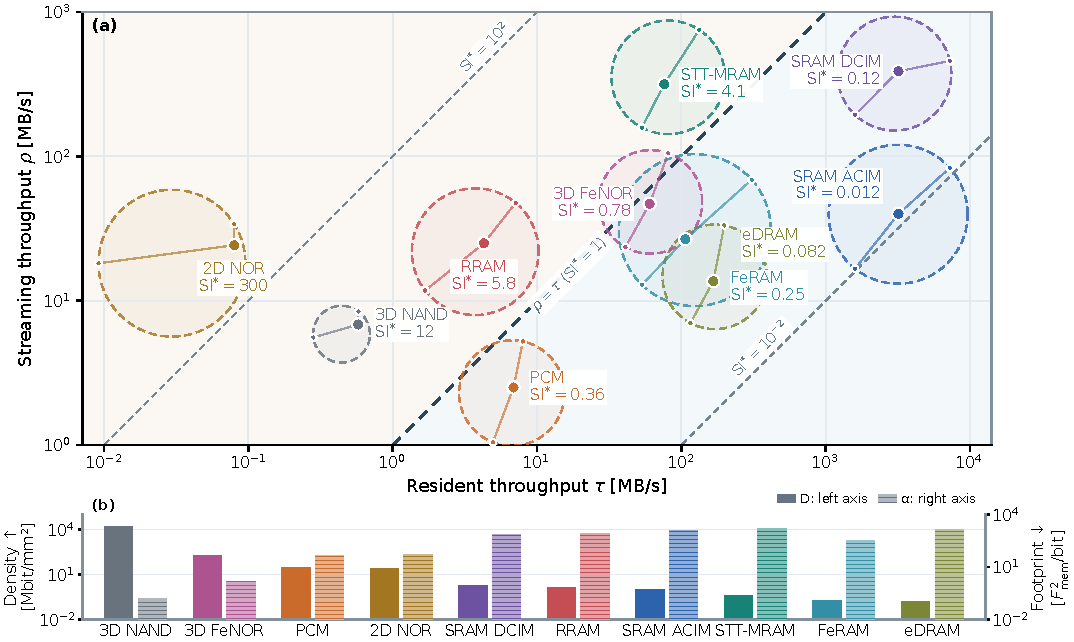
\includegraphics[width=\textwidth]{figures/hardware_capacities_paper.pdf}
\caption{Streaming capacity $\rho$ and resident-update capacity $\tau$ for ten native reference configurations; $1\ \mathrm{MB/s}=10^6\ \Byte/\mathrm{s}$. Large points are typical scenarios; small points preserve the original paired alternatives. Circles summarize only those finite scenarios, and $\RI^*=1$ is a capacity-ratio reference, not a universal workload boundary. Native sizes and resources differ.}
\label{fig:hardware-capacities}
\end{paperwidefigure}
\par\medskip
    % Selected from Task II(b) 04_crosscheck/data/results.json; no O-projection values are implied.
\begin{paperwidetable}
\caption{Streaming intensities of representative inference matrix stages}
\label{tab:workload-intensity}
\footnotesize\setlength{\tabcolsep}{1.6pt}\renewcommand{\arraystretch}{1.25}
\begin{tabularx}{\textwidth}{@{}p{0.20\textwidth}*{12}{>{\centering\arraybackslash}X}@{}}
\toprule
& \multicolumn{6}{c}{\textbf{Weight projections}} & \multicolumn{6}{c}{\textbf{Attention}} \\
\cmidrule(lr){2-7}\cmidrule(l){8-13}
& \multicolumn{3}{c}{QKV ($U$)} & \multicolumn{3}{c}{FFN/MoE ($U$)} & \multicolumn{3}{c}{Prefill ($L$)} & \multicolumn{3}{c}{Decode ($L$)} \\
\cmidrule(lr){2-4}\cmidrule(lr){5-7}\cmidrule(lr){8-10}\cmidrule(l){11-13}
Model & $1\Kilo$ & $128\Kilo$ & $1\mathrm{M}$ & $16$ & $1\Kilo$ & $16\Kilo$ & $1\Kilo$ & $8\Kilo$ & $64\Kilo$ & $1\Kilo$ & $8\Kilo$ & $64\Kilo$ \\
\midrule
Qwen3.5-2B & 0.200 & 25.6 & 204.8 & 0.00347 & 0.222 & 3.6 & 6.0 & 34.0 & 258.0 & 10.0 & 66.0 & 514.0 \\
Ministral 3 8B & 0.167 & 21.3 & 170.7 & 0.00167 & 0.107 & 1.7 & 10.0 & 66.0 & 514.0 & 18.0 & 130.0 & 1026.0 \\
Qwen3.6-35B-A3B & 0.111 & 14.2 & 113.8 & 0.0130 & 0.833 & 13.3 & 12.0 & 68.0 & 516.0 & 20.0 & 132.0 & 1028.0 \\
Hy3 (295B) & 0.100 & 12.8 & 102.4 & 0.00477 & 0.306 & 4.9 & 20.0 & 132.0 & 1028.0 & 36.0 & 260.0 & 2052.0 \\
Ling-1T (1000B) & 0.100 & 12.8 & 102.4 & 0.00326 & 0.208 & 3.3 & 20.0 & 132.0 & 1028.0 & 36.0 & 260.0 & 2052.0 \\
MiMo-V2.5-Pro (1020B) & 0.0377 & 4.8 & 38.6 & 0.00347 & 0.222 & 3.6 & 35.2 & 214.4 & 1648.0 & 60.8 & 419.2 & 3286.4 \\
\bottomrule\end{tabularx}
\par\smallskip\raggedright
Entries are $\SI$; all roles use one byte/element. QKV includes any gate, excluding O. FFN/MoE counts one dense FFN or one routed expert. Prefill builds KV from empty; decode appends one token to a visible length $L$. $1\Kilo=1024$, $1\mathrm{M}=1024^2$. Ling-1T at $64\Kilo$ uses the fixed extension.
\end{paperwidetable}
}\fi}
\newcommand{\paperfixedcolumnheight}{%
  \ifpaperfixedpages
    % Page 1 keeps IEEEtran's title-adjusted column height.
    \ifnum\c@page>1
      \global\@colht\textheight
      \ifnum\c@page=2
        \if@firstcolumn\else
          \global\advance\@colht-\dimexpr\ht\paperfigtwobox+\dp\paperfigtwobox
            +\ht\papertableonebox+\dp\papertableonebox+2\paperfixedgap\relax
        \fi
      \fi
      \ifnum\c@page=3
        \global\advance\@colht-\dimexpr\ht\paperfigthreebox+\dp\paperfigthreebox+\paperfixedgap\relax
      \fi
      \ifnum\c@page=4
        \global\advance\@colht-\dimexpr\ht\papertabletwobox+\dp\papertabletwobox+\paperfixedgap\relax
      \fi
      \ifdim\@colht<3\baselineskip
        \PackageError{paper-fixed-layout}{Pinned objects leave insufficient body space}{Reduce the object height.}%
      \fi
    \fi
  \fi}
\AddToHook{cmd/@startcolumn/before}{\paperfixedcolumnheight}
\AddToHook{build/column/after}{%
  \ifpaperfixedpages\ifnum\c@page=2\if@firstcolumn\else
    \setbox\@outputbox=\vbox to\textheight{\offinterlineskip
      \copy\paperfigtwobox\vskip\paperfixedgap
      \box\@outputbox\vskip\paperfixedgap\vfill
      \copy\papertableonebox}%
  \fi\fi\fi}
\AddToHook{build/page/before}{%
  \ifpaperfixedpages
    \ifnum\c@page=3
      \setbox\@outputbox=\vbox{\offinterlineskip
        \copy\paperfigthreebox\vskip\paperfixedgap\box\@outputbox}%
    \fi
    \ifnum\c@page=4
      \setbox\@outputbox=\vbox{\offinterlineskip
        \copy\papertabletwobox\vskip\paperfixedgap\box\@outputbox}%
    \fi
  \fi}
\ifpaperfixedpages
  % Obsolete draft breaks must not counteract the page reservations.
  \renewcommand{\draftcolumnbreak}{}%
  \renewcommand{\draftpagebreak}{}%
\fi
\makeatother
